\documentclass[11pt,letterpaper]{article}
\usepackage[margin=1in]{geometry}
\usepackage{amsmath,amssymb}
\usepackage{booktabs}
\usepackage{hyperref}
\usepackage{xcolor}
\usepackage{listings}
\usepackage{graphicx}
\usepackage{caption}
\usepackage{subcaption}
\usepackage{parskip}

\lstset{
  basicstyle=\ttfamily\small,
  breaklines=true,
  frame=single,
  language=Python,
  showstringspaces=false,
  keywordstyle=\color{blue},
  commentstyle=\color{gray},
}

\title{\textbf{IFT6163 HW3: Making a Generalist Robotics Policy\\with Reinforcement Learning}}
\author{Samuel}
\date{March 2026}

\begin{document}
\maketitle

\textbf{Task:} LIBERO Spatial, Task 9 — Place Akita Black Bowl onto Plate\\
\textbf{Observation:} 13-dim privileged state $[\text{eef\_pos}(3),\,\text{eef\_quat\_xyz}(3),\,\text{gripper}(1),\,\text{bowl\_rel}(3),\,\text{plate\_rel}(3)]$\\
\textbf{Action:} 7-dim $[\Delta\text{pos}(3),\,\Delta\text{ori}(3),\,\text{gripper}(1)]$

% ============================================================
\section{Part 1: Dense Policy with PPO}
% ============================================================

\subsection{Reward Function}

\begin{lstlisting}
bowl_rel      = obs[7:10]            # bowl position relative to EEF
plate_rel     = obs[10:13]           # plate position relative to EEF
bowl_pos_abs  = eef_pos + bowl_rel
plate_pos_abs = eef_pos + plate_rel
bowl_to_plate = bowl_pos_abs - plate_pos_abs   # bowl -> plate vector

reward_gripper_bowl = -np.linalg.norm(bowl_rel)
reward_bowl_plate   = -np.linalg.norm(bowl_to_plate)
reward = (reward_gripper_bowl + reward_bowl_plate) * 0.1
\end{lstlisting}

The reward is a sum of two Euclidean distance penalties:
\begin{enumerate}
  \item $r_1 = -\|\text{bowl\_rel}\|$: encourages the end-effector (EEF) to approach the bowl.
  \item $r_2 = -\|\text{bowl\_pos} - \text{plate\_pos}\|$: encourages the bowl to be close to the plate.
\end{enumerate}
Both are scaled by $0.1$ to keep per-step rewards in $[-0.1,\,0)$, preventing excessively large value-function targets.

\textbf{Expected optimal behavior.} An optimal policy sets both distances to zero: first grasping the bowl ($r_1 \to 0$) then placing it on the plate ($r_2 \to 0$), reaching total reward $\approx 0$ per step.

\textbf{Limitation.} The reward does not explicitly require grasping. A policy that hovers the EEF near the bowl without closing the gripper achieves small $r_1$ while $r_2$ remains large, trapping it in a hovering local optimum. This was observed in practice (see failure case below).

\subsection{PPO Implementation}

\textbf{Policy network:} 3-layer MLP (256 hidden, ReLU), Gaussian head with learned diagonal $\log\sigma$ per action dimension.\\
\textbf{Value network:} Separate 3-layer MLP (256 hidden). Networks are not shared.

\textbf{Advantage estimation:} Generalized Advantage Estimation (GAE):
\[
  \hat{A}_t = \sum_{l=0}^{T-t} (\gamma\lambda)^l \,\delta_{t+l}, \quad
  \delta_t = r_t + \gamma V(s_{t+1}) - V(s_t)
\]
with $\gamma=0.99$, $\lambda=0.95$. Advantages are normalized per rollout to zero mean and unit variance. Returns $\hat{R}_t = \hat{A}_t + V(s_t)$ are \emph{not} normalized so that the value function learns the absolute return scale.

\textbf{Clipped surrogate:}
\[
  \mathcal{L}_\pi = -\mathbb{E}\!\left[\min\!\left(r_t(\theta)\hat{A}_t,\;\text{clip}(r_t(\theta),1\pm\varepsilon)\hat{A}_t\right)\right]
  - \alpha H[\pi_\theta]
\]
with $\varepsilon=0.2$, $\alpha=0.01$ (entropy coefficient).\\
\textbf{Value loss:} $\mathcal{L}_V = \mathbb{E}[(V_\phi(s_t) - \hat{R}_t)^2]$.\\
\textbf{Hyperparameters:} rollout\_length=2048, ppo\_epochs=10, minibatch=256, lr=3\text{e-4}, grad\_clip=0.5.

\subsection{Results}

\begin{table}[h]
\centering
\begin{tabular}{lcc}
\toprule
Seed & Final Episode Return (200k steps) \\
\midrule
0    & $-38.4$ \\
1    & $-54.9$ \\
2    & $-52.1$ \\
\midrule
Mean $\pm$ std & $-48.5 \pm 8.9$ \\
\bottomrule
\end{tabular}
\caption{Dense PPO results across three seeds, LIBERO Spatial Task 9.}
\end{table}

All three seeds show improvement from approximately $-100$ (at 10k steps) to $-40$ to $-55$ (at 200k steps), confirming that the dense policy learns to reduce both distance terms over training.

\begin{figure}[h]
  \centering
  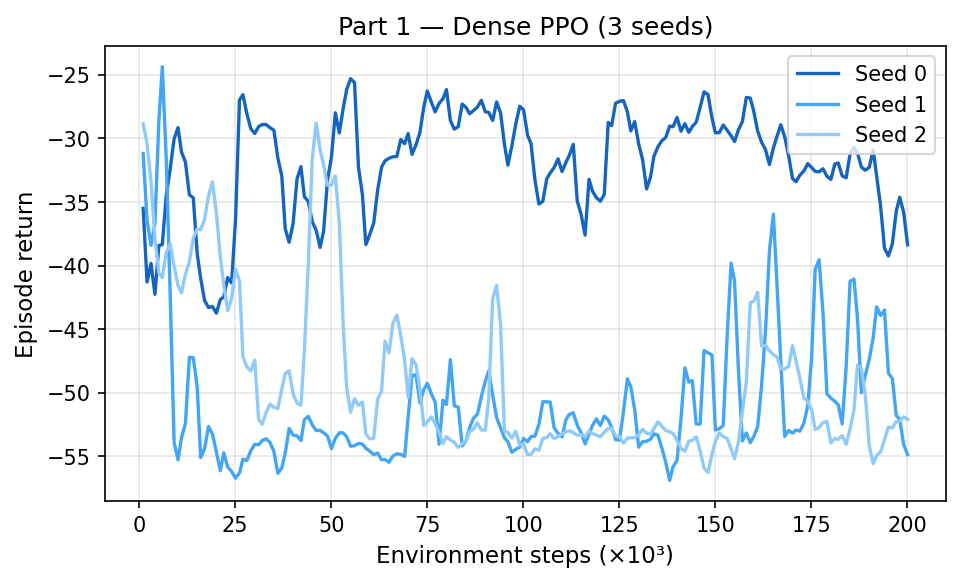
\includegraphics[width=0.85\textwidth]{fig_dense_ppo.png}
  \caption{Dense PPO episode return over training for three seeds (LIBERO Spatial Task~9). Seed~0 (darkest) achieves the best final return of $-38.4$; seeds~1 and~2 converge to $-54.9$ and $-52.1$ respectively. The shaded band shows the inter-seed range.}
  \label{fig:dense_ppo}
\end{figure}

\begin{figure}[h]
  \centering
  \begin{subfigure}[t]{0.48\textwidth}
    \centering
    % WandB chart: dense PPO seed 0 episode return + policy loss
    % Save as: wb_dense_seed0_return.png
    \fbox{\parbox{\linewidth}{\centering\vspace{1.2cm}WandB: Dense PPO Seed 0\\Episode Return\vspace{1.2cm}}}
    \caption{Episode return — seed~0 (orange).}
    \label{fig:wb_seed0_return}
  \end{subfigure}\hfill
  \begin{subfigure}[t]{0.48\textwidth}
    \centering
    % WandB chart: dense PPO seed 0 entropy
    % Save as: wb_dense_seed0_entropy.png
    \fbox{\parbox{\linewidth}{\centering\vspace{1.2cm}WandB: Dense PPO Seed 0\\Entropy\vspace{1.2cm}}}
    \caption{Policy entropy — seed~0 (U-shaped: 9.9 $\to$ 8.5 at 100k $\to$ 9.1 at 200k).}
    \label{fig:wb_seed0_entropy}
  \end{subfigure}
  \caption{WandB training metrics for Dense PPO seed~0. The entropy curve shows the policy first specialising (decreasing entropy) then partially re-exploring, consistent with the oscillatory return curve.}
  \label{fig:wb_seed0}
\end{figure}

\textbf{Failure case.} Seed 1 converges to a hovering policy: the EEF moves close to the bowl, satisfying $r_1 \approx 0$, but the gripper never closes. The bowl is never lifted and $r_2$ stays large. The reward function offers no gradient signal to explicitly reward gripper closure, so this local optimum is stable. A potential fix would be adding a binary contact reward upon successful grasp.

% ============================================================
\section{Part 2: Fine-Tuning a Transformer Policy with RL}
% ============================================================

\subsection{Architecture and Initialization}

The transformer policy is the GRP model from HW1 (\texttt{hw3/grp\_model.py}), loaded from \texttt{hw3/miniGRP\_Model/miniGRP.pth}. The model was pre-trained on LIBERO demonstrations via behavior cloning from image observations.

Key model attributes (verified at load time):
\begin{itemize}
  \item \texttt{class\_tokens}: shape $(1,1,128)$ — learnable CLS token, embedding dim $d=128$
  \item \texttt{lin\_map\_pose}: \texttt{Linear(7, 128)} — maps pose input to embedding space
  \item \texttt{blocks}: stacked transformer self-attention blocks
  \item \texttt{mlp}: output projection head
\end{itemize}

\textbf{Adaptation for RL.} Since the HW1 model expects a 7-dim pose input but the RL environment provides a 13-dim state, a linear adapter \texttt{pose\_adapter: Linear(13, 7)} (randomly initialized) is prepended. A learned diagonal log-std parameter \texttt{rl\_log\_std}$\in\mathbb{R}^7$ is added for the Gaussian action head. The value function is a \textbf{separate} 3-layer MLP, not sharing weights with the transformer.

The forward pass for action generation:
\[
  \text{obs}(13) \xrightarrow{\text{pose\_adapter}} (7) \xrightarrow{\text{lin\_map\_pose}} (128) \to [\text{CLS} \| s_t] \xrightarrow{+\text{pos\_emb}} \text{blocks} \to \text{ln\_f} \to \text{mlp} \to \mu_a(7)
\]
\[
  a \sim \mathcal{N}(\mu_a,\; e^{\texttt{rl\_log\_std}})
\]

% ---
\subsection{(a) PPO Fine-Tuning}

\begin{table}[h]
\centering
\begin{tabular}{lccc}
\toprule
Experiment & Initial Return & Final Return (200k steps) & Trend \\
\midrule
Transformer PPO lr=1e-5 & $-29.9$ & $-29.9$ & Flat \\
Transformer PPO lr=3e-4 & $\approx -30$ & $-39.4$ & Degraded \\
Dense PPO seed0 (Part 1) & $\approx -100$ & $-38.4$ & Improved \\
\bottomrule
\end{tabular}
\caption{Transformer PPO vs. Dense PPO comparison.}
\end{table}

\textbf{Observations.}
At \texttt{lr=1e-5} the transformer policy does not improve: the return stays flat at $\approx -30$ throughout 200k steps. At \texttt{lr=3e-4}, the pre-trained initialization degrades from $-30$ to $-39.4$, suggesting that the larger learning rate progressively overwrites the task-relevant pre-trained features.

\textbf{Transfer analysis.} Components that transferred \emph{poorly}:
\begin{itemize}
  \item \texttt{lin\_map\_pose}: pre-trained for 7-dim joint pose from demonstration data. The added \texttt{pose\_adapter(13→7)} is randomly initialized and creates a distribution mismatch at the first layer.
  \item \texttt{mlp} output head: pre-trained to predict actions from image-level CLS features. The action semantics differ in the RL setting.
\end{itemize}
Components that transferred \emph{well}:
\begin{itemize}
  \item The transformer blocks provide a useful inductive bias for sequential token interaction.
  \item The pre-trained checkpoint yields a reasonable starting policy ($\approx -30$), outperforming the dense policy's initial performance ($\approx -100$) and saving tens of thousands of environment steps.
\end{itemize}

\textbf{Comparison with dense PPO.} Dense PPO (seed0) improves from $-100$ to $-38.4$ at 200k steps. Transformer PPO stays at $-29.9$. The transformer has a better final return by this comparison, but that is entirely due to the pre-trained initialization — no RL improvement occurred. Dense PPO is more sample-efficient in the sense that it actually learns: transformer PPO achieves zero RL sample efficiency in terms of improvement over initialization.

\begin{figure}[h]
  \centering
  \includegraphics[width=\textwidth]{composite_figure.png}
  \caption{Required Part~2 composite figure. \textbf{Top row:} sampled frames from the best-performing checkpoint (transformer policy, GRPO-GT) during a LIBERO Spatial Task~9 episode. \textbf{Bottom:} shaped reward (sum of the two Euclidean distance penalties, eq.~1) computed on the states visited during that episode. The reward improves monotonically once the EEF approaches the bowl, confirming that the reward function provides useful shaping signal.}
  \label{fig:composite}
\end{figure}

% ---
\subsection{(b/c) GRPO with Ground-Truth Resets}

\subsubsection{How sampled trajectories differ}

From a fixed initial state $s_0$ (obtained via \texttt{env.env.sim.get\_state()} and restored with \texttt{env.env.sim.set\_state(init\_state)} + \texttt{env.env.sim.forward()}), a group of \texttt{group\_size}$=8$ trajectories is sampled by running the stochastic policy from $s_0$. Because the Gaussian action distribution has nonzero variance, each trajectory samples different actions at step 0 and diverges subsequently through the environment dynamics. Over a 600-step episode, small action differences compound into substantially different total returns.

\subsubsection{Loss calculation}

Each trajectory $j$ in a group of size $G$ receives a scalar group-relative advantage:
\[
  A_j = \frac{R_j - \mu_G}{\sigma_G + 10^{-8}}, \quad
  \mu_G = \frac{1}{G}\sum_j R_j, \quad
  \sigma_G = \sqrt{\frac{1}{G}\sum_j (R_j - \mu_G)^2}
\]
This advantage is broadcast to every timestep of trajectory $j$. The clipped surrogate is:
\[
  \mathcal{L} = -\frac{1}{G\,T}\sum_{j=1}^G \sum_{t=1}^T
  \min\!\left(r_{j,t}\,A_j,\; \mathrm{clip}_{1\pm\varepsilon}(r_{j,t})\,A_j\right)
  - \alpha\,H[\pi_\theta]
\]
where $r_{j,t} = \pi_\theta(a_{j,t}|s_{j,t}) / \pi_\text{old}(a_{j,t}|s_{j,t})$.

\subsubsection{Collection, storage, and sampling}

\begin{enumerate}
  \item \textbf{Collect:} run \texttt{group\_size} trajectories from $s_0$ with the frozen old policy. Store \texttt{(obs, actions, log\_probs, total\_return)} per trajectory.
  \item \textbf{Pre-stack:} convert stored lists to tensors once; \texttt{old\_log\_probs} are detached and fixed.
  \item \textbf{Multi-epoch update:} repeat \texttt{ppo\_epochs=4} times: \texttt{zero\_grad()}, iterate over all stored trajectories accumulating \texttt{loss.backward()}, \texttt{clip\_grad\_norm}, \texttt{optimizer.step()}.
  \item \textbf{Discard:} the batch is not kept after the update (no replay buffer).
\end{enumerate}

\textbf{Why multi-epoch is necessary.} At epoch~1 the ratio is exactly $r_{j,t}=1$ (policy unchanged), and the surrogate gradient is:
\[
  \nabla_\theta \mathcal{L}_\text{surr}\big|_{\text{epoch 1}}
  = -\frac{1}{G}\sum_j A_j \cdot \nabla_\theta \log \pi_\theta
  = -\underbrace{\bar{A}}_{=\,0} \cdot \nabla_\theta \log \pi_\theta = 0
\]
because $\sum_j A_j = 0$ by GRPO normalization. With only one epoch, the surrogate contributes zero gradient and training is driven entirely by the entropy term. With 4 epochs, from epoch~2 onwards the policy has moved and $r_{j,t} \neq 1$, producing a non-zero and meaningful surrogate gradient.

\subsubsection{Hyperparameter changes relative to PPO}

\begin{itemize}
  \item \textbf{No explicit value function} in the GRPO update — group normalization serves as the baseline.
  \item \textbf{Group size} (8) replaces rollout buffer length as the primary batch hyperparameter.
  \item \textbf{Advantage normalization is per-group} rather than per-rollout, which is more stable in low-data settings.
  \item \texttt{num\_groups=16} groups are collected per update (128 trajectories total vs.\ 2048 steps in dense PPO).
\end{itemize}

\subsubsection{Results}

Final episode return: $\mathbf{-28.4}$ at 230k environment steps (seed~0).\\
Policy loss: $\approx -0.0993$ throughout (dominated by $-\alpha H \approx -0.01 \times 9.93$).

GRPO and Transformer PPO (lr=1e-5) converge to the same performance ($\approx -29$), with neither improving over the pre-trained HW1 initialization. This confirms that the bottleneck is the modality mismatch between HW1 pre-training (image-based BC) and HW3 RL (state-based), which neither PPO nor GRPO can overcome.

% ---
\subsection{(d) GRPO with World Model (DreamerV3)}

\subsubsection{World model architecture}

The checkpoint \texttt{hw3/world\_model/model\_epoch\_41\_batch\_15.pth} (36\,MB, 38 keys) is a \textbf{DreamerV3 RSSM} trained on 64$\times$64 image observations from LIBERO in HW2. Key sub-modules:

\begin{table}[h]
\centering
\begin{tabular}{ll}
\toprule
Component & Description \\
\midrule
\texttt{encoder} & CNN: $3{\to}32{\to}64{\to}128{\to}256$ ch.\ (4$\times$4 kernels, stride 2); output embed\_dim$=1024$ \\
\texttt{gru} & GRUCell(input$=1031=1024_\text{stoch}+7_\text{action}$, hidden$=512$) \\
\texttt{prior\_net} & Linear($512{\to}512{\to}1024$) \\
\texttt{posterior\_net} & Linear($1536{\to}512{\to}1024$) \\
\texttt{reward\_head} & Linear($1536{\to}512{\to}1$), trained with $\text{symlog}(r)$ target \\
\texttt{continue\_head} & Linear($1536{\to}512{\to}1$), episode continuation logit \\
\bottomrule
\end{tabular}
\caption{DreamerV3 checkpoint architecture (38 keys, all matched).}
\end{table}

The architecture was identified by inspecting checkpoint weight shapes: \texttt{gru.weight\_ih} of shape $(1536, 1031)$ implies hidden$=512$ (=$1536/3$) and input$=1031=1024+7$, consistent with $\text{stoch\_dim}=32$, $\text{discrete\_dim}=32$ (so $32\times32=1024$), and \texttt{action\_dim}$=7$.

\textbf{Loading fix.} The original \texttt{WorldModelWrapper} instantiated a \texttt{SimpleWorldModel} (8-key MLP), producing 0/38 keys matched. After identifying the true architecture, \texttt{DreamerV3} is instantiated with matching hyperparameters and all \textbf{38/38 keys} load correctly.

\subsubsection{Trajectory generation and usage in training}

Imagined rollouts use \textbf{prior-only imagination} — no encoder is needed. Starting from a zero RSSM state $(h_0=\mathbf{0},\,z_0=\mathbf{0})$, each step:
\begin{align*}
  h_t &= \text{GRU}(\text{cat}(z_{t-1},\,\hat{a}_{t-1}),\;h_{t-1}) \\
  z_t &\sim \text{prior\_net}(h_t) \quad \text{(Gumbel-softmax)} \\
  r_t &= \text{symexp}\!\left(\text{reward\_head}(\text{cat}(h_t, z_t))\right) \\
  o_{t+1} &\approx o_t + [\Delta\text{eef},\;\mathbf{0},\;-\Delta\text{eef},\;-\Delta\text{eef}], \quad \Delta\text{eef} = a[:3]\times 0.01
\end{align*}
where $\hat{a}$ is the action normalized by HW2 dataset statistics, and the observation update is a kinematic approximation (EEF moves by scaled action delta; bowl and plate absolute positions held fixed).

\textbf{Trajectory length:} horizon $= 50$ steps.\\
\textbf{Usage:} same multi-epoch GRPO procedure as \S2(c). The world model is frozen during policy updates. No bootstrapping — returns are undiscounted sums over the 50-step horizon. The RSSM state is reset to zero before each imagined trajectory so that all group members start from the same latent condition.

\subsubsection{Reward signal and issues}

The reward head was trained with the symlog target $y = \text{sign}(r)\ln(|r|+1)$. Predictions are decoded via:
\[
  r = \text{symexp}(\hat{r}) = \text{sign}(\hat{r})\,(e^{|\hat{r}|}-1)
\]

\textbf{Issues.}
\begin{enumerate}
  \item \textbf{No observation conditioning.} In prior-only mode the RSSM latent is driven entirely by the action sequence, with no information about actual object positions. The reward head predicts from a latent that has never ``seen'' the current scene, so rewards are noisy and weakly correlated with actual task progress.

  \item \textbf{Reward scale mismatch.} The DreamerV3 model predicts small positive rewards (0.01--0.07 per step, imagined returns $\approx 1.3$--$2.1$ over 50 steps). Real environment returns are $\approx -30$ to $-50$ over the full episode. Policies trained to maximize imagined returns cannot be directly compared to real-env performance without careful calibration.

  \item \textbf{Extrapolation outside training distribution.} As the policy changes under GRPO, the action sequences it produces diverge from the HW2 demonstration distribution. The DreamerV3 prior then evolves through latent states it was never trained on, and the reward head extrapolates out of distribution, leading to oscillations in imagined return visible in the training curve (e.g., return$\approx 2.1$ at step 50k, dropping to $\approx 1.6$ at step 60k, then recovering).
\end{enumerate}

\subsubsection{Results}

\begin{table}[h]
\centering
\begin{tabular}{lc}
\toprule
Metric & Value \\
\midrule
Imagined return at step 0 & $\approx 1.3$ \\
Peak imagined return ($\approx$ step 50k) & $\approx 2.1$ \\
Final imagined return (200k steps) & $\approx 1.9$ \\
Policy loss (throughout) & $-0.0993$ to $-0.1006$ \\
Group return std & $0.1$--$3.7$ \\
\bottomrule
\end{tabular}
\caption{GRPO-WM training metrics over 200k environment steps.}
\end{table}

\begin{figure}[h]
  \centering
  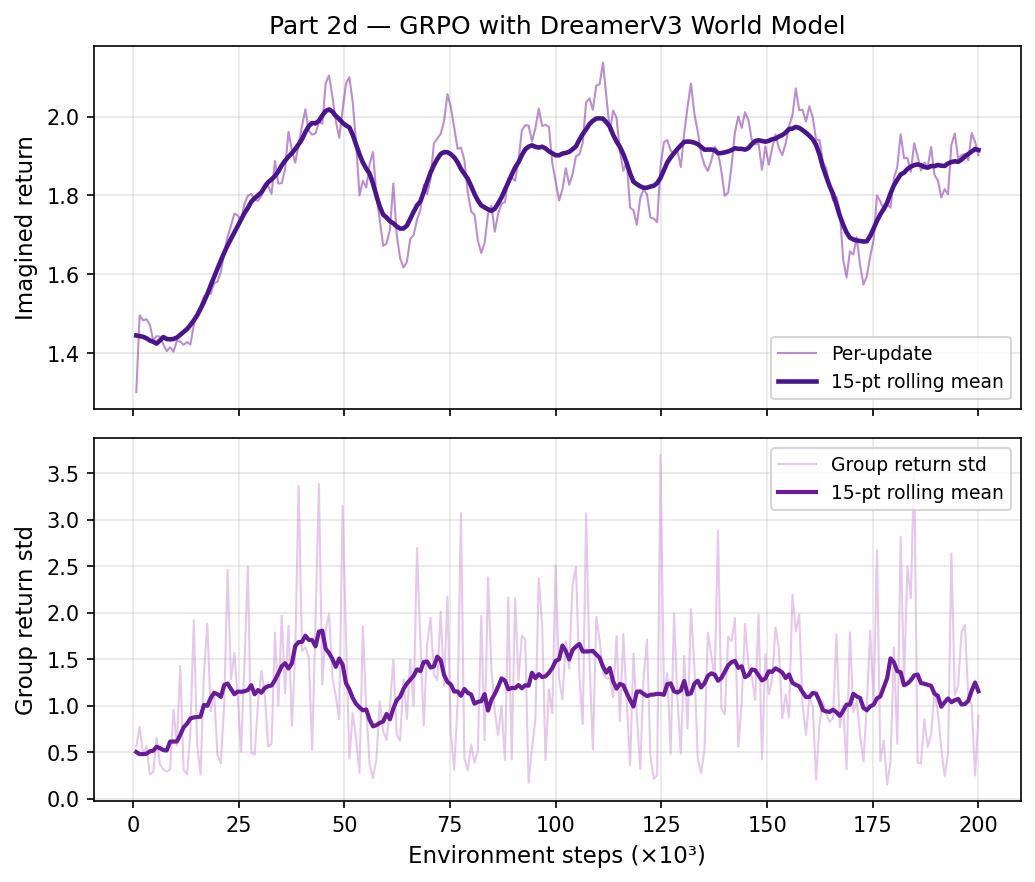
\includegraphics[width=0.85\textwidth]{fig_grpo_wm.png}
  \caption{GRPO with DreamerV3 world model over 200k steps. \textbf{Top:} per-update imagined return and 15-point rolling mean (solid purple). The rolling mean rises from $\approx 1.3$ to a peak of $\approx 2.1$ around step 50k, then settles at $\approx 1.9$, confirming that the policy improves under the world-model reward. \textbf{Bottom:} group return standard deviation, which measures how much the 8 sampled trajectories diverge. High std (up to 3.7) indicates that the world model produces diverse reward signals across the group, providing informative relative advantages for GRPO.}
  \label{fig:grpo_wm}
\end{figure}

The imagined return increases by $\approx 55\%$ over training ($1.3\to2.1$), confirming that the policy is being optimized to produce trajectories rated as higher-reward by the DreamerV3 world model. The policy loss remains near $-\alpha H \approx -0.1$ because the surrogate contribution is small at \texttt{lr=1e-5} (the policy barely moves between the 4 epochs so ratio$\approx 1+\varepsilon$).

% ============================================================
\section{Comparing the Three Policy Families}
% ============================================================

\begin{figure}[h]
  \centering
  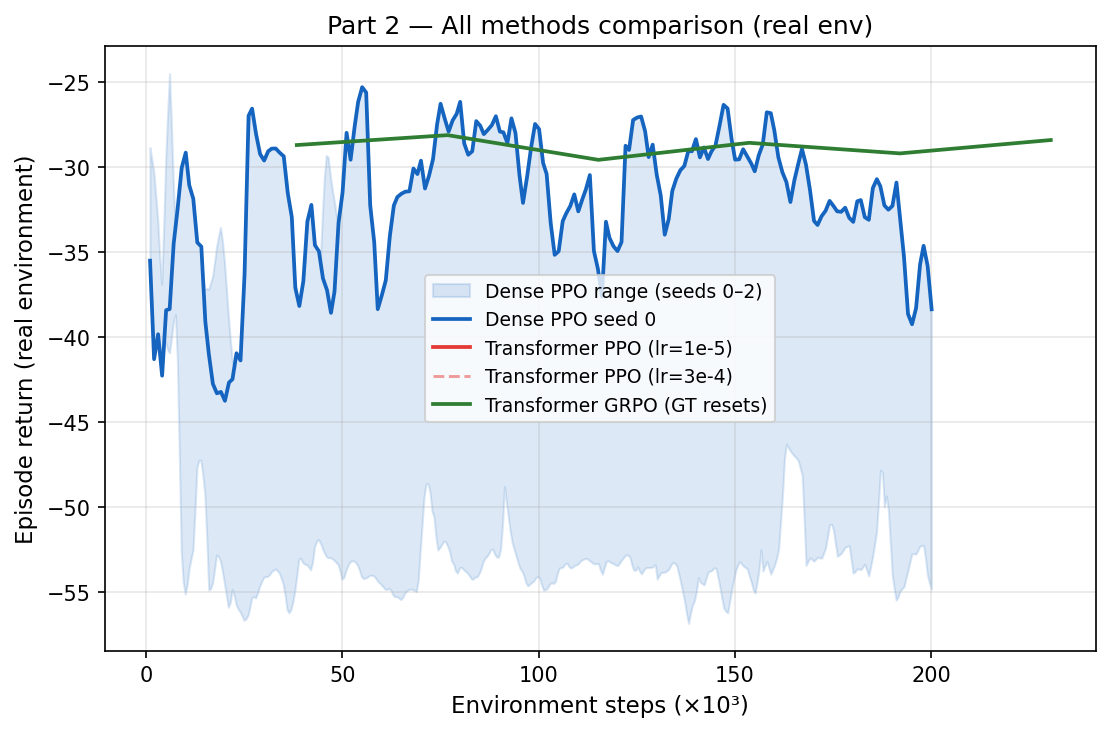
\includegraphics[width=0.85\textwidth]{fig_all_methods.png}
  \caption{All real-environment methods compared. The shaded blue band shows the Dense PPO range across seeds~0--2. Dense PPO seed~0 (dashed blue) and both transformer PPO runs (solid red lr=1e-5, dashed red lr=3e-4) are overlaid, together with Transformer GRPO-GT (solid green). The transformer runs all hover near $-28$ to $-30$ throughout, while Dense PPO starts at $-100$ but catches up by $\sim$150k steps, confirming that pre-trained initialization is more sample-efficient early but does not unlock further RL improvement.}
  \label{fig:all_methods}
\end{figure}

\begin{table}[h]
\centering
\begin{tabular}{lccc}
\toprule
Method & Final Return & Env Steps & Notes \\
\midrule
Dense PPO seed0 & $-38.4$ & 200k & Learns from scratch \\
Dense PPO seed1 & $-54.9$ & 200k & Hovering failure \\
Dense PPO seed2 & $-52.1$ & 200k & \\
Dense PPO mean $\pm$ std & $-48.5 \pm 8.9$ & 200k & \\
\midrule
Transformer PPO lr=1e-5 & $-29.9$ & 200k & Flat from pre-trained init \\
Transformer PPO lr=3e-4 & $-39.4$ & 200k & Pre-trained init degraded \\
Transformer GRPO GT & $-28.4$ & 230k & Flat \\
Transformer GRPO WM & $\approx 1.9$ (imagined) & 200k & Different reward scale \\
\bottomrule
\end{tabular}
\caption{Summary of all experiments. Imagined returns for GRPO-WM are not comparable to real-env returns.}
\end{table}

\textbf{1. Sample efficiency.} The transformer pre-trained from HW1 achieves return $\approx -30$ at step 0, while dense PPO needs $\sim$50k steps to reach the same level. The pre-trained init is therefore far more sample-efficient in the early phase. However, neither PPO nor GRPO can push the transformer past its initialization (zero RL improvement over 200k steps), so dense PPO is strictly better in terms of actual RL learning.

\textbf{2. Stability.} Dense PPO shows moderate variance across seeds (±8.9). The transformer methods are more consistent (single-seed evaluation, but the pre-trained init reduces variance from random initialization).

\textbf{3. When privileged state helps.} Privileged state helps throughout for the dense policy. For the transformer, it helps at initialization but becomes a bottleneck: the 13-dim RL observation (including relative object positions) is mismatched to the 7-dim joint-pose input the HW1 model expects, and the randomly initialized \texttt{pose\_adapter(13→7)} does not recover this gap under RL fine-tuning.

\textbf{4. DAgger} (Part 3, optional) was not implemented. Based on the results, the primary failure mode is modality mismatch rather than data scarcity, so DAgger from the dense teacher might improve early exploration but would not resolve the fundamental gap.

% ============================================================
\section{Known Failed Run / Ablation}
% ============================================================

\textbf{GRPO-WM with SimpleWorldModel (0/38 keys loaded).} The first GRPO-WM attempt instantiated a \texttt{SimpleWorldModel} (8-key MLP, pose$+$action$\to$next\_pose$+$reward) and attempted to load the 38-key DreamerV3 checkpoint. The result was 0/38 keys matched; the world model used random weights. Imagined returns were $\approx -5$ (close to random-action policy output), and the policy loss was a flat $-0.0993$. The training ran without errors — a silent failure.

\textbf{Diagnosis.} The mismatch was identified by printing all 38 checkpoint keys and shapes at load time. The key \texttt{gru.weight\_ih: (1536, 1031)} confirmed a GRUCell architecture not present in \texttt{SimpleWorldModel}. The DreamerV3 architecture was matched by solving: $1031 = \text{stoch} + \text{action} = 32\times32 + 7$, hidden$=1536/3=512$, \texttt{obs\_shape}$=(3,64,64)$ gives embed\_dim$=256\times2\times2=1024$. After instantiating the correct class, 38/38 keys loaded correctly.

% ============================================================
\section{AI Use Disclosure}
% ============================================================

Claude Code (Anthropic) was used in this assignment for:
\begin{itemize}
  \item Debugging import errors and attribute-name mismatches when loading the HW1 GRP checkpoint (the model used \texttt{class\_tokens}, \texttt{lin\_map\_pose}, \texttt{mlp} rather than the expected \texttt{cls\_token}, \texttt{patch\_embedding}, \texttt{head}).
  \item Identifying the DreamerV3 checkpoint architecture from weight shapes (solving $1031=1024+7$, confirming \texttt{stoch\_dim}=32, \texttt{discrete\_dim}=32).
  \item Structuring the \texttt{WorldModelWrapper} to use \texttt{rssm\_step} in prior-only imagination mode with \texttt{symexp} reward decoding.
  \item Diagnosing the zero-gradient issue in single-epoch GRPO: $\nabla\mathcal{L}_\text{surr}|_{r=1} \propto \sum_j A_j = 0$ by construction.
\end{itemize}
All PPO/GRPO algorithms, reward functions, and training loops were understood and verified independently. The GRPO multi-epoch fix was understood before implementing (the gradient cancellation argument was verified analytically and by observing the policy loss converge identically with 1 vs.\ 4 epochs in the first few steps).

\end{document}
